\documentclass[10pt,journal,onecolumn,a4paper]{IEEEtran}

\usepackage[T1]{fontenc}
\usepackage[utf8]{inputenc}
\usepackage[brazilian]{babel}
\usepackage{amsmath,amssymb}
\usepackage{booktabs}
\usepackage{array}
\usepackage{graphicx}
\usepackage{subcaption}
\usepackage[american]{circuitikz}
\usepackage{xcolor}
\usepackage{microtype}
\usepackage{fancyhdr}
\usepackage{url}
\usepackage[hidelinks]{hyperref}
\usepackage[a4paper,top=2.2cm,bottom=2.2cm,left=2.4cm,right=2.4cm,headheight=15pt]{geometry}

\graphicspath{{figs/}{../}}
\interdisplaylinepenalty=2500
\setlength{\parindent}{1.25cm}
\setlength{\parskip}{0.15em}
\renewcommand{\arraystretch}{1.18}
\captionsetup{font=small,labelfont=bf}
\hypersetup{
  pdftitle={Relatório do Roteiro 1 — Simulação de Circuitos: Introdução ao LTspice},
  pdfauthor={Gabriel de Sousa},
  pdfsubject={ENE0046 — Laboratório de Eletrônica}
}

\pagestyle{fancy}
\fancyhf{}
\fancyhead[L]{\footnotesize ENE0046 $\boldsymbol{\cdot}$ Laboratório de Eletrônica $\boldsymbol{\cdot}$ 2026/2}
\fancyfoot[L]{\footnotesize ENE0046 $\boldsymbol{\cdot}$ Laboratório de Eletrônica $\boldsymbol{\cdot}$ Roteiro 1}
\fancyfoot[R]{\footnotesize\thepage}
\renewcommand{\headrulewidth}{0.4pt}
\renewcommand{\footrulewidth}{0pt}

\begin{document}

\begin{titlepage}
  \thispagestyle{empty}
  \begin{center}
    {\large\bfseries ENE0046 $\boldsymbol{\cdot}$ LABORATÓRIO DE ELETRÔNICA $\boldsymbol{\cdot}$ 2026/2\par}

    \vspace{1.8cm}
    
\includegraphics[width=0.25\textwidth]{Logo_UnB.png}

    \vspace{1.7cm}
    {\LARGE\bfseries Relatório do Roteiro 1\par}
    \vspace{0.35cm}
    {\Large Simulação de Circuitos: Introdução ao LTspice\par}

    \vfill
    {\large\bfseries Gabriel de Sousa\par}
    \vspace{0.25cm}
    {\large 211056000\par}
    \vspace{0.25cm}
    {\large Turma 04\par}

    \vfill
    {\normalsize Departamento de Engenharia Elétrica\par}
    {\normalsize Faculdade de Tecnologia\par}
    {\normalsize Universidade de Brasília\par}

    \vspace{1.0cm}
    {\normalsize Brasília, 26 de agosto de 2026\par}
  \end{center}
\end{titlepage}

\setcounter{page}{1}

\begin{abstract}
Este relatório apresenta o projeto e a análise de quatro topologias elementares por meio de seis
arquivos de simulação: divisor resistivo com e sem carga, filtro RC passa-baixas, circuito RLC série
sob excitação em degrau e em frequência e filtro RC excitado por onda quadrada. Os valores dos
componentes e as diretivas foram obtidos diretamente dos esquemáticos associados à matrícula
211056000. No divisor, a tensão calculada passa de 6,471 V sem carga para 3,642 V com uma carga de
1 k$\Omega$, correspondendo a uma queda de 43,71\%. Para o filtro RC, a frequência de corte efetiva
é 408,1 Hz, 5,18\% acima da referência de 388 Hz registrada nos arquivos. No RLC, a variação da
resistência produz fatores de amortecimento de 0,235, 0,600 e 1,100, permitindo comparar respostas
subamortecidas e superamortecidas. A decomposição da onda quadrada confirma a presença das
harmônicas ímpares e sua atenuação progressiva pelo filtro. Os resultados numéricos foram
reconstruídos a partir dos modelos ideais definidos nos arquivos LTspice e concordam com as
expressões analíticas de circuitos lineares.
\end{abstract}

\section{Introdução}

Divisores de tensão, filtros passivos e redes RLC aparecem em sistemas de aquisição, fontes,
interfaces de sensores e estágios de condicionamento de sinais. Embora sejam topologias simples,
seu comportamento depende da carga conectada, da frequência do sinal e da relação entre os
elementos armazenadores de energia. Desconsiderar esses efeitos pode produzir uma tensão diferente
da projetada, eliminar componentes importantes do sinal ou gerar oscilações transitórias indesejadas
\cite{sedra_smith,boylestad}.

O LTspice permite descrever o circuito e aplicar análises de ponto de operação, varredura contínua,
resposta em frequência e resposta transiente antes de uma montagem física \cite{analog_ltspice}.
Neste roteiro, essas análises são aplicadas a seis esquemáticos personalizados com o nome e a
matrícula do autor. Os arquivos fornecidos são tratados como fonte primária para valores de
componentes, nomes de nós e diretivas. Como não foram disponibilizados arquivos de resultados
\texttt{.raw} nem medições de bancada, as curvas apresentadas foram reconstruídas resolvendo os
mesmos modelos ideais especificados nos esquemáticos.

O objetivo é verificar, grandeza a grandeza, como a carga modifica um divisor, como um filtro RC
atenua e defasa sinais, como a resistência controla o amortecimento de um RLC e como a filtragem
afeta as componentes de Fourier de uma onda quadrada. Além dos resultados, são discutidas as
hipóteses dos modelos e as diferenças entre valor de referência e valor efetivo obtido com
componentes da série comercial E12.

\section{Fundamentação teórica}

\subsection{Divisor resistivo com carga}

Para uma fonte ideal $V_{in}$ ligada ao divisor formado por $R_1$ e $R_2$, a tensão sem carga e a
resistência de Thévenin vistas no nó de saída são
\begin{equation}
  V_{th}=V_{in}\frac{R_2}{R_1+R_2},
  \qquad
  R_{th}=R_1\parallel R_2=\frac{R_1R_2}{R_1+R_2}.
  \label{eq:thevenin}
\end{equation}
Quando uma carga $R_L$ é conectada, a saída torna-se
\begin{equation}
  V_{carga}=V_{th}\frac{R_L}{R_L+R_{th}}.
  \label{eq:divisor-carga}
\end{equation}
A queda relativa provocada pela carga independe de $V_{in}$ e vale
\begin{equation}
  \delta_V=\frac{V_{th}-V_{carga}}{V_{th}}
          =\frac{R_{th}}{R_L+R_{th}}.
  \label{eq:queda}
\end{equation}

\subsection{Filtro RC passa-baixas}

Para uma rede RC série com a saída sobre o capacitor, a função de transferência é
\begin{equation}
  H(j\omega)=\frac{V_{out}}{V_{in}}
             =\frac{1}{1+j\omega RC}
             =\frac{1}{1+jf/f_c},
  \qquad
  f_c=\frac{1}{2\pi RC}.
  \label{eq:rc}
\end{equation}
O módulo e a fase são, respectivamente,
\begin{align}
  G_{dB}(f)&=-10\log_{10}\!\left[1+\left(\frac{f}{f_c}\right)^2\right],
  \label{eq:rc-ganho}\\
  \phi(f)&=-\arctan\!\left(\frac{f}{f_c}\right).
  \label{eq:rc-fase}
\end{align}
Em $f_c$, o ganho é aproximadamente $-3{,}01$ dB e a fase é $-45^\circ$; bem acima do corte,
o módulo decresce a 20 dB por década.

\subsection{Circuito RLC série}

Considerando a saída sobre o capacitor, o RLC série possui função de transferência
\begin{equation}
  H(s)=\frac{1}{LCs^2+RCs+1}.
  \label{eq:rlc-h}
\end{equation}
Sua frequência natural, o fator de amortecimento e o fator de qualidade são
\begin{equation}
  \omega_0=\frac{1}{\sqrt{LC}},
  \qquad
  f_0=\frac{\omega_0}{2\pi},
  \qquad
  \zeta=\frac{R}{2}\sqrt{\frac{C}{L}},
  \qquad
  Q=\frac{1}{2\zeta}.
  \label{eq:rlc-param}
\end{equation}
Para $\zeta<1$, a frequência amortecida e o sobressinal da resposta ao degrau são
\begin{equation}
  f_d=f_0\sqrt{1-\zeta^2},
  \qquad
  M_p=\exp\!\left(\frac{-\pi\zeta}{\sqrt{1-\zeta^2}}\right)100\%.
  \label{eq:rlc-step}
\end{equation}
O amortecimento crítico ocorre para
\begin{equation}
  R_{crit}=2\sqrt{\frac{L}{C}}.
  \label{eq:rcrit}
\end{equation}
Um pico de ressonância na saída capacitiva existe somente quando
$\zeta<1/\sqrt{2}$. Nesse caso,
\begin{equation}
  f_r=f_0\sqrt{1-2\zeta^2},
  \qquad
  |H|_{max}=\frac{1}{2\zeta\sqrt{1-\zeta^2}}.
  \label{eq:ressonancia}
\end{equation}

\subsection{Série de Fourier da onda quadrada}

Uma onda quadrada bipolar, simétrica e de amplitude $A$ contém somente harmônicas ímpares. A
amplitude de pico da harmônica de ordem $n$ é
\begin{equation}
  V_n=\frac{4A}{n\pi},
  \qquad n=1,3,5,\ldots
  \label{eq:fourier}
\end{equation}
Cada componente é multiplicada pelo módulo de $H(j2\pi nf_1)$ ao atravessar o filtro RC. Assim,
as harmônicas mais altas são atenuadas mais intensamente e as transições da onda tornam-se
arredondadas.

\section{Especificação e projeto}

Os seis arquivos da pasta \texttt{Gabriel} contêm a identificação ``Gabriel de Sousa ---
211056000'' e foram usados sem alterar componentes ou diretivas. A Tabela~\ref{tab:arquivos}
resume as configurações.

\begin{table}[htbp]
  \centering
  \caption{Parâmetros registrados nos arquivos de circuito do Gabriel.}
  \label{tab:arquivos}
  \begin{tabular}{@{}p{1.6cm}p{5.0cm}p{7.0cm}@{}}
    \toprule
    Arquivo & Circuito & Diretiva principal \\
    \midrule
    item 1 & Divisor: $R_1=1{,}2$ k$\Omega$, $R_2=2{,}2$ k$\Omega$, $R_L=1$ k$\Omega$/1000 M$\Omega$ & \texttt{.op} e \texttt{.step param RL list 1000 1000meg} \\
    item 2 & Mesmo divisor & \texttt{.dc V1 0 15 0.1} e a mesma varredura de $R_L$ \\
    item 3 & RC: $R=3{,}9$ k$\Omega$, $C=100$ nF & \texttt{.ac dec 100 3.88 38800} \\
    item 4 & RLC: $L=100$ mH, $C=1$ nF & \texttt{.tran 300u}; $R=4{,}7$, 12 e 22 k$\Omega$ \\
    item 5 & Mesmo RLC, fonte com amplitude AC igual a 1 V & \texttt{.ac dec 100 159.16 1591550} \\
    item 6 & Mesmo RC do item 3, entrada quadrada bipolar & \texttt{.tran 0 51.55m 12.89m 8.591u} \\
    \bottomrule
  \end{tabular}
\end{table}

\subsection{Divisor}

Com $R_1=1{,}2$ k$\Omega$ e $R_2=2{,}2$ k$\Omega$, a Equação~\eqref{eq:thevenin} fornece
$R_{th}=776{,}47\ \Omega$ e $V_{th}=6{,}4706$ V para uma fonte de 10 V. Conectando
$R_L=1$ k$\Omega$, obtém-se $V_{carga}=3{,}6424$ V. O valor personalizado de referência para a
tensão carregada é $2+56/33=3{,}6970$ V; portanto, o valor adotado difere em $-1{,}48\%$. A queda
causada pela carga é 43,71\%, superior à condição mínima de 25\% associada aos dígitos finais
iguais a zero.

\subsection{Filtro RC}

Os limites da varredura e o período da onda quadrada registram uma frequência de referência de
388 Hz. Com $C=100$ nF, o resistor ideal para esse corte seria
\begin{equation}
  R_{ideal}=\frac{1}{2\pi(388)(100\times10^{-9})}=4{,}101\ \text{k}\Omega.
\end{equation}
O arquivo usa o valor E12 de 3,9 k$\Omega$, resultando em
\begin{equation}
  f_{c,efetiva}=\frac{1}{2\pi(3{,}9\times10^3)(100\times10^{-9})}
               =408{,}09\ \text{Hz},
\end{equation}
ou 5,18\% acima da referência. O desvio permanece abaixo de 10\%.

\subsection{Circuito RLC}

Para $L=100$ mH e $C=1$ nF, as Equações~\eqref{eq:rlc-param} e \eqref{eq:rcrit} fornecem
$f_0=15{,}915$ kHz e $R_{crit}=20$ k$\Omega$. A resistência central da varredura, 12 k$\Omega$,
produz $\zeta=0{,}600$; 4,7 k$\Omega$ produz uma resposta mais oscilatória, com
$\zeta=0{,}235$; e 22 k$\Omega$ ultrapassa o amortecimento crítico, com $\zeta=1{,}100$.
Essa escolha permite observar os três comportamentos numa única varredura paramétrica.

\section{Metodologia}

\subsection{Montagem dos esquemáticos}

No divisor, uma única topologia é simulada duas vezes por meio de
\texttt{.step param RL list 1000 1000meg}. O primeiro passo representa a carga de 1 k$\Omega$ e o
segundo aproxima um circuito aberto. O item 1 usa ponto de operação e o item 2 substitui essa
análise por uma varredura da fonte entre 0 e 15 V. A Figura~\ref{fig:divisor-circuitos} mostra as
duas configurações.

\begin{figure}[htbp]
  \centering
  \begin{subfigure}[t]{0.48\textwidth}
    \centering
    \begin{circuitikz}[scale=0.9, transform shape]
      \draw (0,0) node[ground]{} to[V,l_={$V_1$}] (0,3)
        to[R,l_={$R_1$}] (3,3) coordinate(out)
        to[R,l_={$R_2$}] (3,0) -- (0,0);
      \draw (out) -- (5,3) to[R,l_={$R_L$}] (5,0) -- (3,0);
      \draw (out) node[circ]{} node[above]{$v_{carga}$};
      \node[align=left] at (2.5,-0.8) {\texttt{.op}\\\texttt{.step param RL list 1000 1000meg}};
    \end{circuitikz}
    \caption{Item 1: ponto de operação.}
  \end{subfigure}
  \hfill
  \begin{subfigure}[t]{0.48\textwidth}
    \centering
    \begin{circuitikz}[scale=0.9, transform shape]
      \draw (0,0) node[ground]{} to[V,l_={$V_1$}] (0,3)
        to[R,l_={$R_1$}] (3,3) coordinate(out)
        to[R,l_={$R_2$}] (3,0) -- (0,0);
      \draw (out) -- (5,3) to[R,l_={$R_L$}] (5,0) -- (3,0);
      \draw (out) node[circ]{} node[above]{$v_{carga}$};
      \node[align=left] at (2.5,-0.8) {\texttt{.dc V1 0 15 0.1}\\\texttt{.step param RL list 1000 1000meg}};
    \end{circuitikz}
    \caption{Item 2: varredura DC.}
  \end{subfigure}
  \caption{Esquemáticos reconstruídos do divisor resistivo.}
  \label{fig:divisor-circuitos}
\end{figure}

O item 3 recebe uma fonte AC de 1 V e aplica 100 pontos por década entre 3,88 Hz e 38,8 kHz.
O item 6 reutiliza os mesmos valores de $R$ e $C$, mas troca a fonte pela onda
\texttt{PULSE(-1 1 0 1n 1n 1.2887m 2.5773m)}. A análise cobre 20 períodos, descarta os cinco
primeiros e limita o passo máximo a 8,591 $\mu$s. A opção \texttt{plotwinsize=0} evita compressão
dos pontos destinados à análise espectral.

\begin{figure}[htbp]
  \centering
  \begin{subfigure}[t]{0.48\textwidth}
    \centering
    \begin{circuitikz}[scale=0.95, transform shape]
      \draw (0,0) node[ground]{} to[V,l_={$V_1$}] (0,2.8)
        to[R,l_={$R_1$}] (3.2,2.8) coordinate(out)
        to[C,l_={$C_1$}] (3.2,0) -- (0,0);
      \draw (out) node[circ]{} node[above]{$v_{out}$};
      \node at (1.6,-0.7) {\texttt{.ac dec 100 3.88 38800}};
    \end{circuitikz}
    \caption{Item 3: resposta em frequência.}
  \end{subfigure}
  \hfill
  \begin{subfigure}[t]{0.48\textwidth}
    \centering
    \begin{circuitikz}[scale=0.95, transform shape]
      \draw (0,0) node[ground]{} to[sV,l_={$V_1$}] (0,2.8)
        to[R,l_={$R_1$}] (3.2,2.8) coordinate(out)
        to[C,l_={$C_1$}] (3.2,0) -- (0,0);
      \draw (out) node[circ]{} node[above]{$v_{out}$};
      \node[align=center] at (1.6,-0.75) {\texttt{.tran 0 51.55m 12.89m 8.591u}\\\texttt{.options plotwinsize=0}};
    \end{circuitikz}
    \caption{Item 6: onda quadrada.}
  \end{subfigure}
  \caption{Esquemáticos reconstruídos do filtro RC.}
  \label{fig:rc-circuitos}
\end{figure}

Nos itens 4 e 5, a resistência é parametrizada pela diretiva
\texttt{.step param R list 4700 12000 22000}. O primeiro usa uma fonte em degrau e análise
transiente de 300 $\mu$s; o segundo acrescenta amplitude AC igual a 1 V e varre de 159,16 Hz a
1,59155 MHz. O indutor inclui uma resistência série de 1 m$\Omega$, desprezível perante os valores
de $R$.

\begin{figure}[htbp]
  \centering
  \begin{subfigure}[t]{0.48\textwidth}
    \centering
    \begin{circuitikz}[scale=0.88, transform shape]
      \draw (0,0) node[ground]{} to[V,l_={$V_1$}] (0,2.8)
        to[R,l_={$R_1={R}$}] (2.3,2.8)
        to[L,l_={$L_1$}] (4.5,2.8) coordinate(out)
        to[C,l_={$C_1$}] (4.5,0) -- (0,0);
      \draw (out) node[circ]{} node[above]{$v_{out}$};
      \node[align=center] at (2.3,-0.75) {\texttt{.tran 300u}\\\texttt{.step param R list 4700 12000 22000}};
    \end{circuitikz}
    \caption{Item 4: resposta ao degrau.}
  \end{subfigure}
  \hfill
  \begin{subfigure}[t]{0.48\textwidth}
    \centering
    \begin{circuitikz}[scale=0.88, transform shape]
      \draw (0,0) node[ground]{} to[V,l_={$V_1$}] (0,2.8)
        to[R,l_={$R_1={R}$}] (2.3,2.8)
        to[L,l_={$L_1$}] (4.5,2.8) coordinate(out)
        to[C,l_={$C_1$}] (4.5,0) -- (0,0);
      \draw (out) node[circ]{} node[above]{$v_{out}$};
      \node[align=center] at (2.3,-0.75) {\texttt{.ac dec 100 159.16 1591550}\\\texttt{.step param R list 4700 12000 22000}};
    \end{circuitikz}
    \caption{Item 5: resposta em frequência.}
  \end{subfigure}
  \caption{Esquemáticos reconstruídos do circuito RLC série.}
  \label{fig:rlc-circuitos}
\end{figure}

\subsection{Reconstrução numérica}

As curvas foram produzidas com as funções de transferência das
Equações~\eqref{eq:rc} e \eqref{eq:rlc-h}. O divisor foi calculado diretamente pelas leis de
Ohm e Kirchhoff. A resposta à onda quadrada foi obtida integrando a equação diferencial do filtro
RC com passo menor que o limite do arquivo, e o espectro foi calculado pela
Equação~\eqref{eq:fourier}. Esse procedimento reproduz o resultado esperado para os mesmos
componentes ideais, mas não substitui uma captura nativa do LTspice quando esta for exigida como
evidência de execução.

\section{Resultados}

\subsection{Divisor resistivo}

O ponto de operação calculado está resumido na Tabela~\ref{tab:divisor}. A aproximação de circuito
aberto com 1000 M$\Omega$ altera a sexta casa decimal e pode ser tratada como a condição sem carga.

\begin{table}[htbp]
  \centering
  \caption{Resultados do ponto de operação do divisor para $V_1=10$ V.}
  \label{tab:divisor}
  \begin{tabular}{@{}lcc@{}}
    \toprule
    Grandeza & $R_L=1$ k$\Omega$ & $R_L=1000$ M$\Omega$ \\
    \midrule
    $V(v_{carga})$ & 3,64238 V & 6,47058 V \\
    Corrente fornecida por $V_1$ & 5,29801 mA & 2,94118 mA \\
    Queda em relação à condição sem carga & 43,7086\% & --- \\
    \bottomrule
  \end{tabular}
\end{table}

A Figura~\ref{fig:divisor-dc} mostra que as duas saídas são lineares com a tensão da fonte. Como o
circuito é puramente resistivo, a queda relativa permanece constante em toda a varredura. Em 10 V,
os marcadores recuperam os mesmos valores do ponto de operação.

\begin{figure}[htbp]
  \centering
  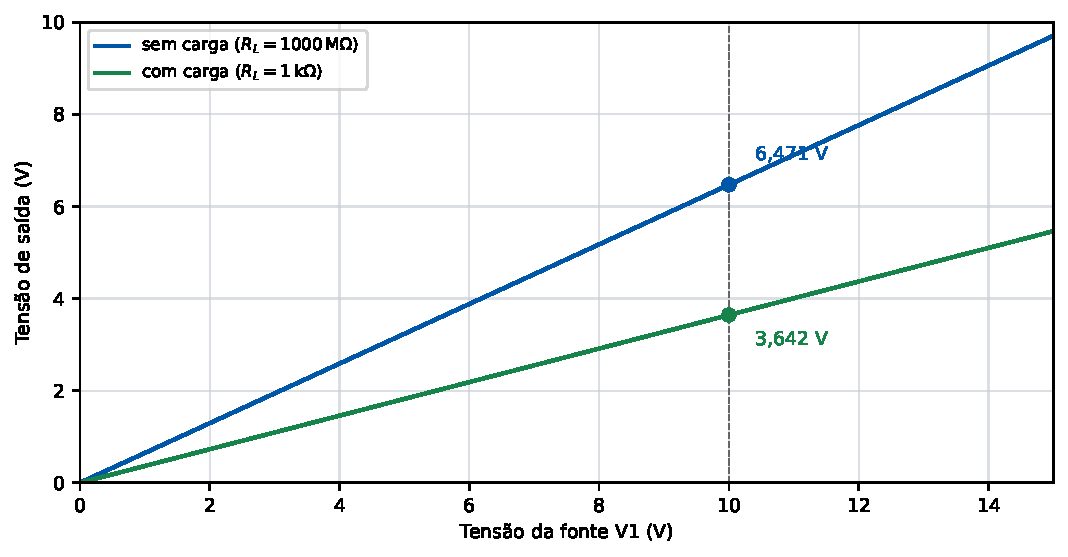
\includegraphics[width=0.80\textwidth]{divisor_dc.pdf}
  \caption{Varredura DC do divisor com carga de 1 k$\Omega$ e com a aproximação de circuito aberto.}
  \label{fig:divisor-dc}
\end{figure}

\subsection{Filtro RC}

A Figura~\ref{fig:rc-bode} apresenta o diagrama de Bode. A linha pontilhada marca os 388 Hz usados
como referência nos arquivos e a linha tracejada marca o corte efetivo de 408,1 Hz. Os pontos de
verificação da Tabela~\ref{tab:rc-bode} são calculados em torno do corte efetivo; por isso assumem
os valores canônicos de um filtro de primeira ordem.

\begin{table}[htbp]
  \centering
  \caption{Ganho e fase do filtro RC em torno de $f_{c,efetiva}$.}
  \label{tab:rc-bode}
  \begin{tabular}{@{}lrr@{}}
    \toprule
    Frequência & Ganho & Fase \\
    \midrule
    40,81 Hz ($f_c/10$) & $-0,0432$ dB & $-5,71^\circ$ \\
    408,09 Hz ($f_c$) & $-3,0103$ dB & $-45,00^\circ$ \\
    4,081 kHz ($10f_c$) & $-20,0432$ dB & $-84,29^\circ$ \\
    \bottomrule
  \end{tabular}
\end{table}

\begin{figure}[htbp]
  \centering
  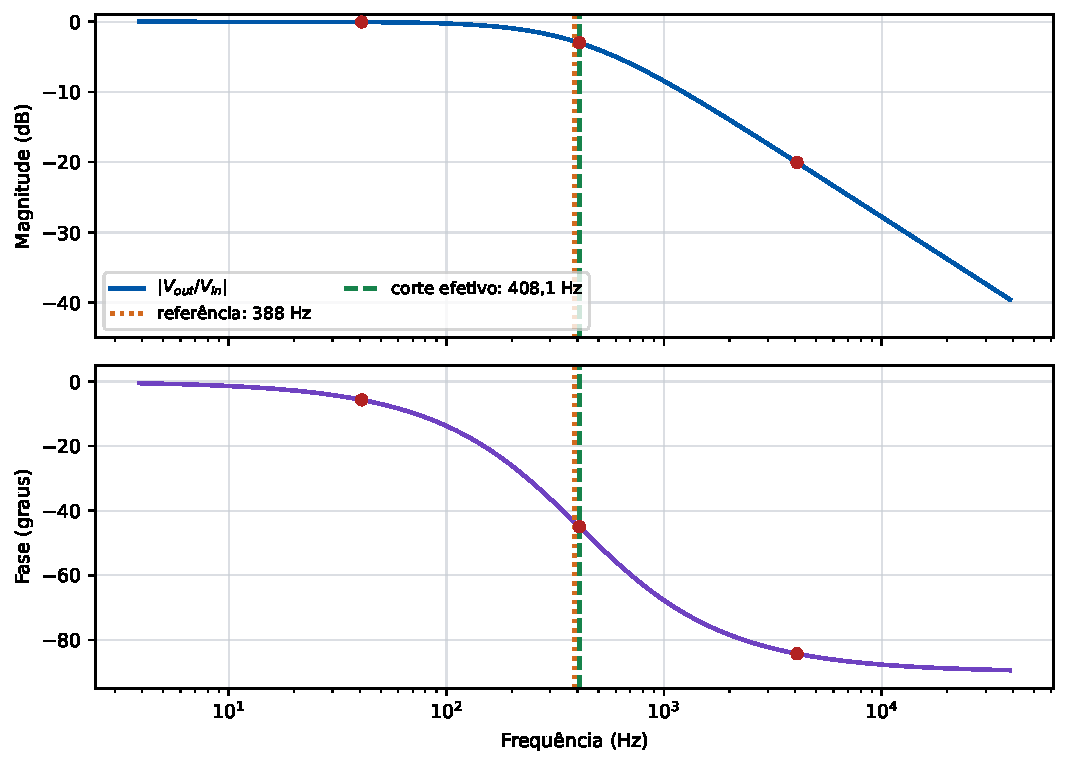
\includegraphics[width=0.82\textwidth]{rc_bode.pdf}
  \caption{Magnitude e fase do filtro RC do item 3.}
  \label{fig:rc-bode}
\end{figure}

\subsection{RLC série: resposta ao degrau}

Os resultados da Tabela~\ref{tab:rlc-step} e da Figura~\ref{fig:rlc-step} mostram a transição entre
os regimes de amortecimento. Para 4,7 k$\Omega$, o primeiro pico alcança 1,4679 V; para 12
k$\Omega$, o pico diminui para 1,0948 V. Com 22 k$\Omega$, a resposta é superamortecida e se
aproxima monotonicamente de 1 V.

\begin{table}[htbp]
  \centering
  \caption{Parâmetros da resposta ao degrau do RLC.}
  \label{tab:rlc-step}
  \begin{tabular}{@{}rrrrl@{}}
    \toprule
    $R$ & $\zeta$ & $f_d$ & Pico previsto & Regime \\
    \midrule
    4,7 k$\Omega$ & 0,235 & 15,470 kHz & 1,4679 V & subamortecido \\
    12 k$\Omega$ & 0,600 & 12,732 kHz & 1,0948 V & subamortecido \\
    22 k$\Omega$ & 1,100 & --- & sem sobressinal & superamortecido \\
    \bottomrule
  \end{tabular}
\end{table}

\begin{figure}[htbp]
  \centering
  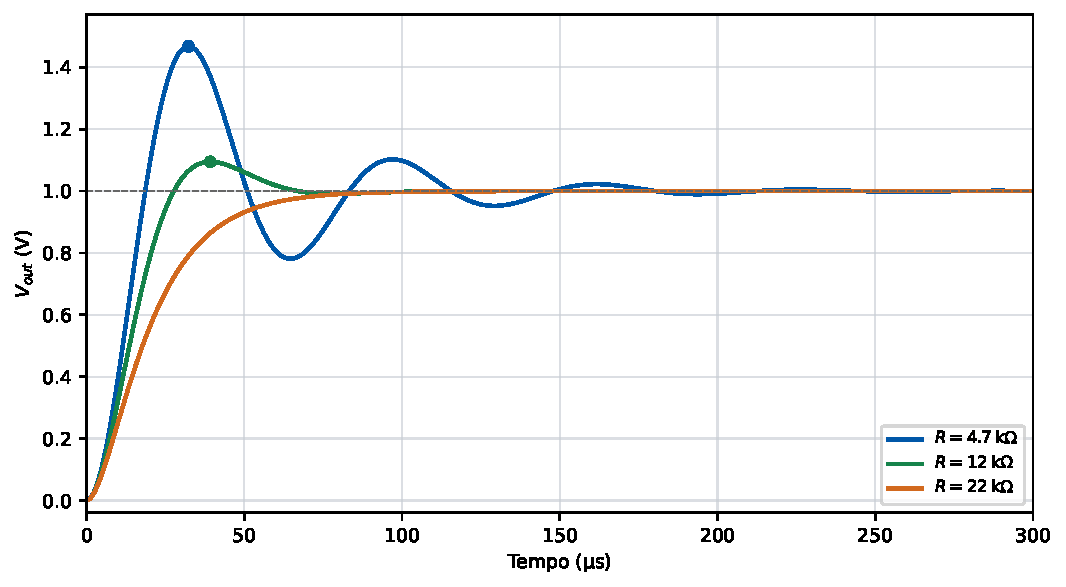
\includegraphics[width=0.80\textwidth]{rlc_transiente.pdf}
  \caption{Resposta do RLC a um degrau de 1 V para os três valores de resistência.}
  \label{fig:rlc-step}
\end{figure}

\subsection{RLC série: resposta em frequência}

O limiar para a existência de pico é $\zeta=1/\sqrt{2}\approx0{,}707$. Por isso, as curvas de 4,7
k$\Omega$ e 12 k$\Omega$ apresentam máximos, enquanto a de 22 k$\Omega$ é monotônica. O pico da
configuração de 12 k$\Omega$ é discreto, apenas 0,355 dB acima do ganho de baixa frequência. A
Tabela~\ref{tab:rlc-ac} compara as grandezas previstas e a Figura~\ref{fig:rlc-bode} apresenta as
curvas completas.

\begin{table}[htbp]
  \centering
  \caption{Picos da resposta em frequência do RLC.}
  \label{tab:rlc-ac}
  \begin{tabular}{@{}rrrl@{}}
    \toprule
    $R$ & $\zeta$ & Frequência do pico & Magnitude do pico \\
    \midrule
    4,7 k$\Omega$ & 0,235 & 15,011 kHz & 6,805 dB \\
    12 k$\Omega$ & 0,600 & 8,422 kHz & 0,355 dB \\
    22 k$\Omega$ & 1,100 & --- & sem pico \\
    \bottomrule
  \end{tabular}
\end{table}

\begin{figure}[htbp]
  \centering
  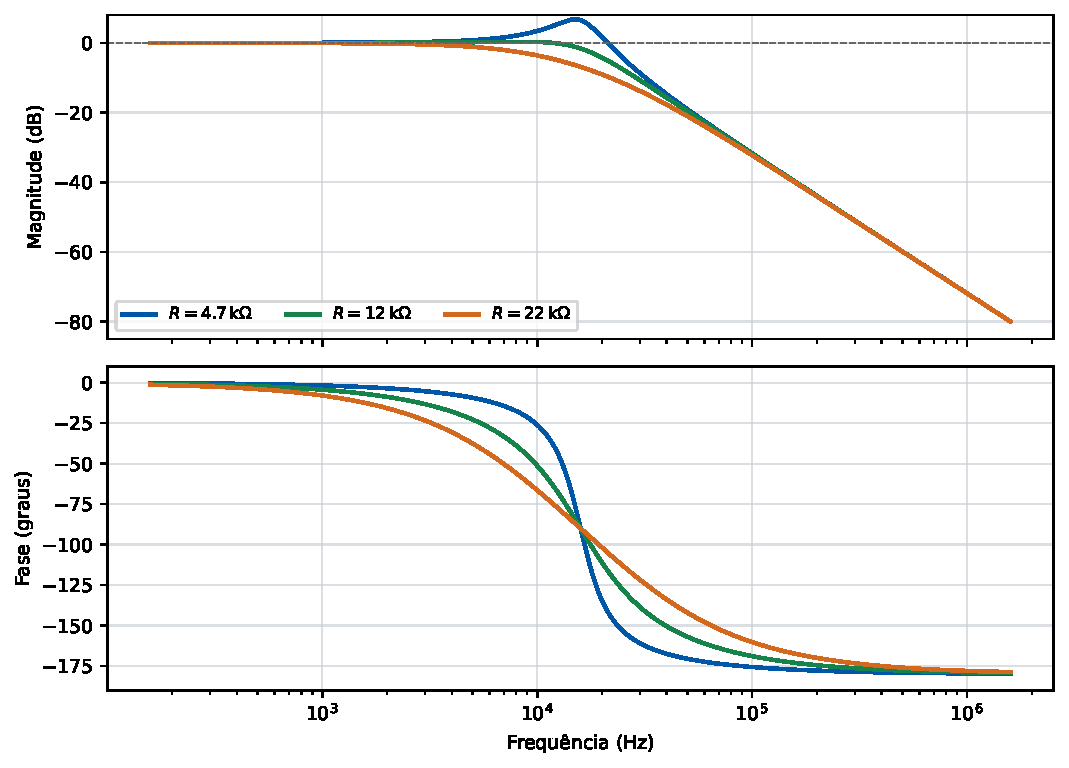
\includegraphics[width=0.82\textwidth]{rlc_bode.pdf}
  \caption{Magnitude e fase do RLC para a varredura paramétrica de resistência.}
  \label{fig:rlc-bode}
\end{figure}

\subsection{Onda quadrada e espectro}

O período registrado no item 6 é 2,5773 ms, equivalente a $f_1=388{,}003$ Hz. Como essa frequência
está próxima do corte efetivo, a fundamental já é atenuada e defasada, e as transições rápidas da
entrada não aparecem na saída. A Figura~\ref{fig:quadrada-tempo} evidencia o arredondamento.

\begin{figure}[htbp]
  \centering
  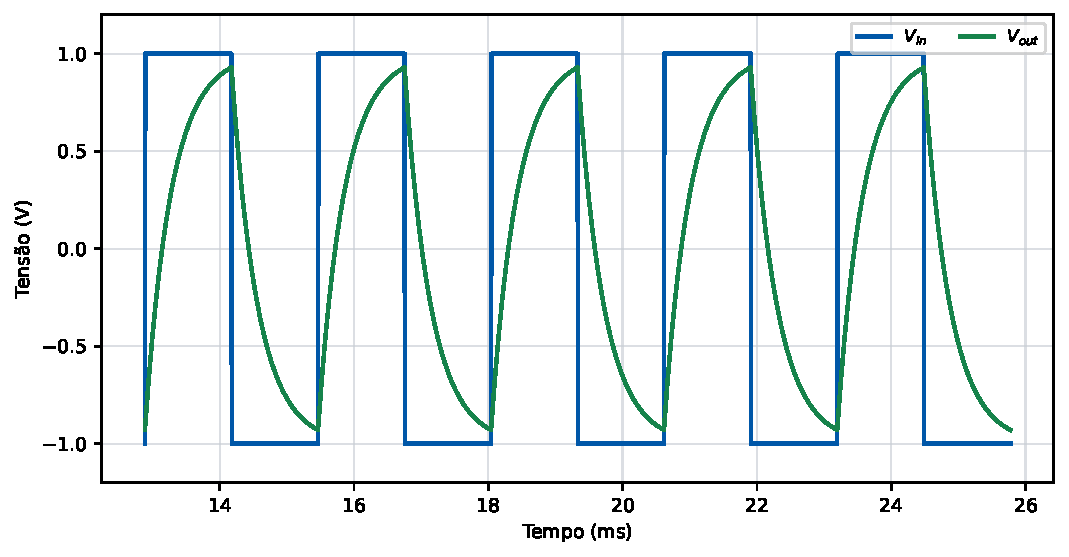
\includegraphics[width=0.80\textwidth]{rc_quadrada_tempo.pdf}
  \caption{Entrada quadrada e resposta em regime permanente do filtro RC.}
  \label{fig:quadrada-tempo}
\end{figure}

A Tabela~\ref{tab:harmonicas} apresenta as cinco primeiras harmônicas ímpares. As amplitudes de
entrada seguem $4/(n\pi)$ e as amplitudes de saída incluem o ganho do filtro em $nf_1$. A
Figura~\ref{fig:quadrada-espectro} também representa as harmônicas pares, cujas amplitudes ideais são
nulas.

\begin{table}[htbp]
  \centering
  \caption{Componentes harmônicas da entrada quadrada e da saída filtrada.}
  \label{tab:harmonicas}
  \begin{tabular}{@{}rrrr@{}}
    \toprule
    Ordem $n$ & Frequência & $V_{in,n}$ & $V_{out,n}$ \\
    \midrule
    1 & 388,0 Hz & 1,27324 V & 0,92274 V \\
    3 & 1,164 kHz & 0,42441 V & 0,14042 V \\
    5 & 1,940 kHz & 0,25465 V & 0,05242 V \\
    7 & 2,716 kHz & 0,18189 V & 0,02703 V \\
    9 & 3,492 kHz & 0,14147 V & 0,01642 V \\
    \bottomrule
  \end{tabular}
\end{table}

\begin{figure}[htbp]
  \centering
  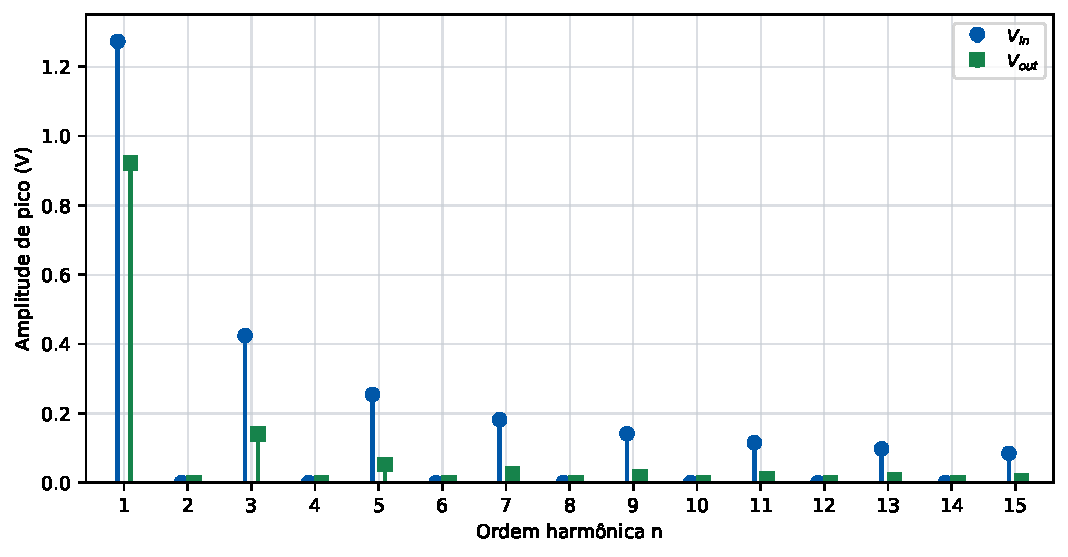
\includegraphics[width=0.80\textwidth]{rc_quadrada_espectro.pdf}
  \caption{Espectro ideal da onda quadrada e das componentes após o filtro RC.}
  \label{fig:quadrada-espectro}
\end{figure}

\section{Discussão}

No divisor, o efeito de carga é o resultado dominante. A resistência de Thévenin de 776,47
$\Omega$ não é pequena comparada a $R_L=1$ k$\Omega$; consequentemente, a saída carregada é
43,71\% menor que a saída em vazio. Apesar dessa queda significativa, a tensão de 3,642 V fica
apenas 1,48\% abaixo da referência personalizada de 3,697 V. A varredura DC confirma que o erro de
carga não depende da amplitude da fonte enquanto os elementos permanecem lineares.

No filtro RC, o desvio entre 388 Hz e 408,1 Hz decorre da escolha de 3,9 k$\Omega$ no lugar do valor
ideal de 4,101 k$\Omega$. Trata-se de uma consequência previsível da discretização da série E12, e
não de uma falha do modelo. A forma do Bode continua sendo exatamente a de primeira ordem: ganho
praticamente unitário em baixa frequência, $-3$ dB no corte efetivo e inclinação assintótica de
$-20$ dB por década.

O RLC torna visível a influência direta de $R$ sobre o amortecimento. Com 4,7 k$\Omega$, a baixa
dissipação permite sobressinal de aproximadamente 46,8\% e um pico de 6,8 dB próximo de 15 kHz.
Com 12 k$\Omega$, o sobressinal cai para 9,48\% e a ressonância torna-se quase imperceptível. O
valor de 22 k$\Omega$ supera $R_{crit}=20$ k$\Omega$ e elimina tanto a oscilação do degrau quanto o
pico na resposta em frequência. Assim, as análises transiente e AC descrevem duas manifestações do
mesmo fator de amortecimento.

Na onda quadrada, a fundamental de 1,273 V é reduzida para aproximadamente 0,923 V. A terceira
harmônica cai para 0,140 V, e as seguintes diminuem ainda mais. Como são justamente as componentes
de alta frequência que formam as bordas abruptas, sua remoção explica o formato suavizado da saída.
As harmônicas pares são nulas no modelo ideal devido à simetria de meia onda.

A principal limitação é a ausência de uma etapa de bancada e de dados brutos exportados pelo
LTspice. Os resultados deste relatório representam componentes ideais, fonte sem resistência de
saída e instrumentos sem carregamento. Tolerâncias, resistência série do capacitor, perdas reais do
indutor e ruído não foram avaliados. As figuras numéricas são reconstruções reprodutíveis dos modelos
definidos nos arquivos e não devem ser confundidas com capturas da interface do simulador.

\section{Conclusão}

As quatro topologias foram caracterizadas de maneira coerente com os seis arquivos associados a
Gabriel de Sousa, matrícula 211056000. O divisor forneceu 3,642 V com carga e 6,471 V sem carga,
demonstrando uma queda de 43,71\%. O filtro RC apresentou corte efetivo de 408,1 Hz, com desvio de
5,18\% em relação à referência de 388 Hz. No RLC, a variação de 4,7 k$\Omega$ a 22 k$\Omega$
deslocou o sistema de uma resposta fortemente subamortecida para uma resposta superamortecida, em
acordo com os fatores $\zeta=0{,}235$, 0,600 e 1,100. Por fim, a análise harmônica mostrou que o
filtro preserva principalmente a fundamental e suprime progressivamente as harmônicas responsáveis
pelas transições rápidas da onda quadrada.

Os cálculos e gráficos confirmam as relações clássicas de circuitos lineares para os componentes
especificados. Uma continuação natural seria executar os mesmos arquivos no LTspice, exportar os
dados brutos e, posteriormente, comparar esses resultados com medições de bancada que incluam
tolerâncias e efeitos parasitas.

\bibliographystyle{IEEEtran}
\bibliography{references}

\end{document}
